\documentclass[25pt, a0paper, portrait]{tikzposter}

\usepackage{polyglossia}

\usepackage{datetime}
\usepackage{fontspec}
\usepackage{microtype}

\setdefaultlanguage{english}
\setmainfont{TeX Gyre Termes}
\usetheme{Simple}
%\usecolorpalette{GreenGrayViolet}

\title{Balancing performance and complexity with adaptive graph coarsening}

\newdate{presentation}{11}{07}{2022}
\date{EEML 2023, \displaydate{presentation}}

\author{Marek Dědič}

\institute{
	Cisco Systems, Inc.,
	Czech Technical University in Prague
}

\begin{document}

\maketitle

\begin{columns}
	\column{0.5}
	\block{The performance-complexity trade-off}{
		\begin{tikzfigure}
			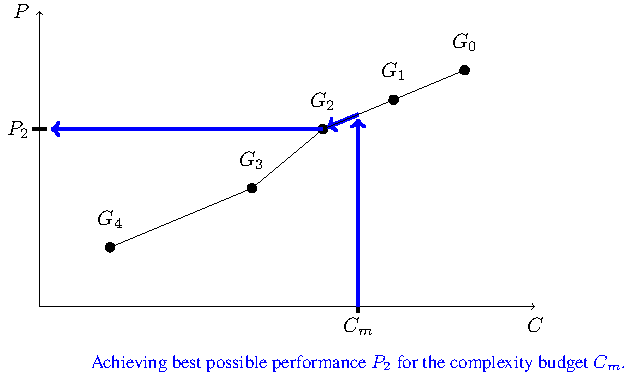
\includegraphics[width=\linewidth]{images/performance-complexity/performance-complexity.pdf}
		\end{tikzfigure}
	}

	\block{Main idea}{
		\begin{tikzfigure}
			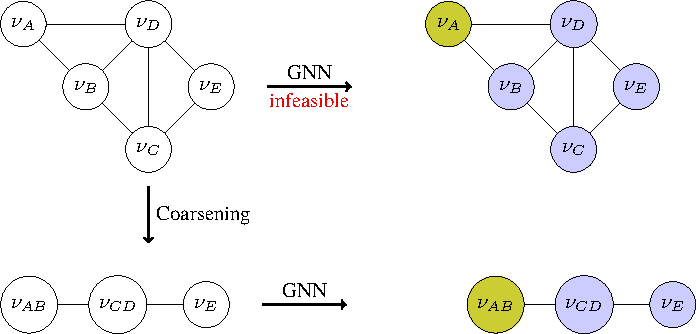
\includegraphics[width=\linewidth]{images/coarsening-illustration/coarsening-illustration.pdf}
		\end{tikzfigure}
	}

	\block{HARP pipeline overview}{
		\begin{tikzfigure}
			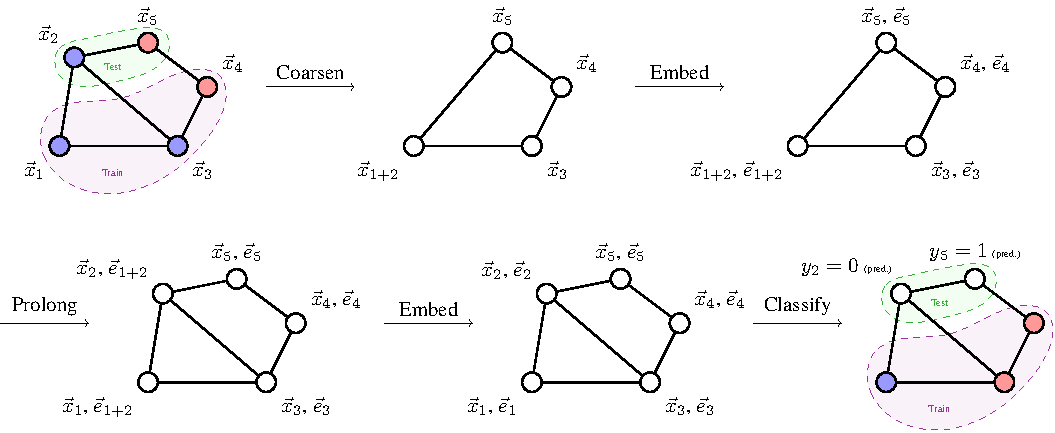
\includegraphics[width=\linewidth]{images/harp-overview/harp-overview.pdf}
		\end{tikzfigure}
	}

	\column{0.5}
	\block{Deep HARP}{
		\begin{tikzfigure}
			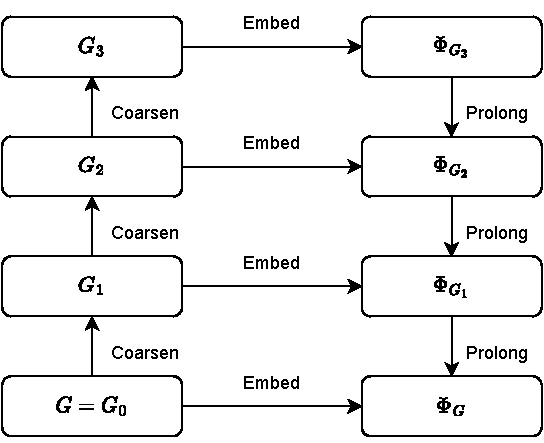
\includegraphics[width=0.5\linewidth]{images/deep-harp/deep-harp.pdf}
		\end{tikzfigure}
	}

	\block{Adaptive prolongation}{
		\begin{tikzfigure}
			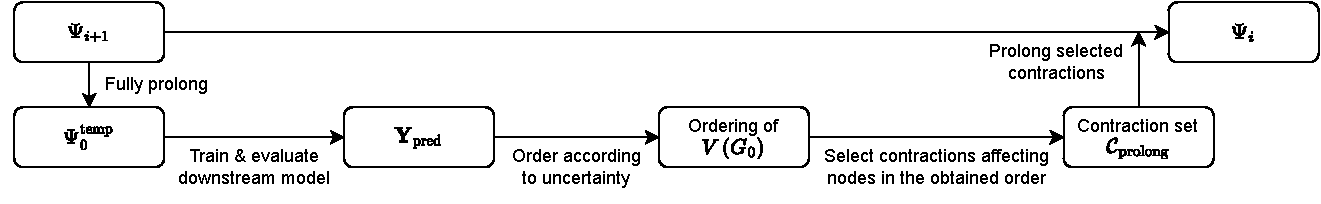
\includegraphics[width=\linewidth]{images/adaptive-prolongation/adaptive-prolongation.pdf}
		\end{tikzfigure}
	}

	\block{Results}{
		\begin{tikzfigure}
			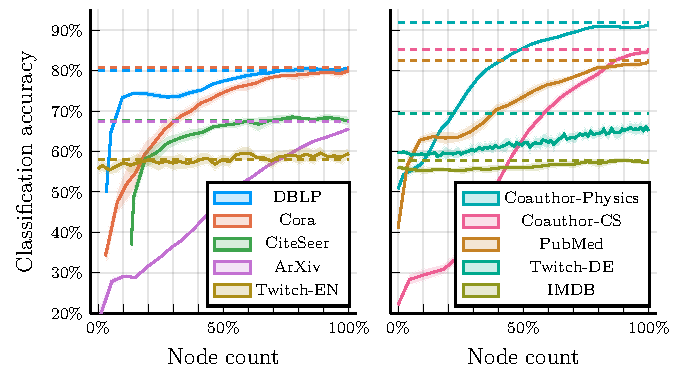
\includegraphics[width = \linewidth]{images/adaptive-coarsening/adaptive-coarsening.pdf}
		\end{tikzfigure}
		Downstream classifier accuracies at different steps of adaptive prolongation. Dashed line shows the baseline node2vec model accuracy. The node count is taken relative to the total node count in each dataset. The results are averaged over multiple runs, with the solid line representing the mean and the shaded area denoting one standard deviation.
	}
\end{columns}

\end{document}
